\section{Background}

\subsection{GPS Positioning}
\begin{figure}
    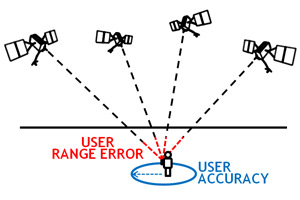
\includegraphics[scale=0.5]{figures/gps-how.jpg}
    \caption{From \cite{gpsGov}: GPS Technology Overview}
\label{fig:gps:how}
\end{figure}


GPS Positioning technology makes use of satelites in known orbits around the earth, broadcasting the current time. By consulting the orbits and the time taken for a signal to arrive from a number of satelites, GPS recievers can determine their own location on Earth, as shown in \figref{fig:gps:how}.

\begin{figure}
    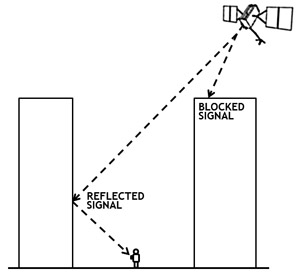
\includegraphics[scale=0.5]{figures/gps-reflect.jpg}
    \caption{From \cite{gpsGov}: GPS sources of error - reflected signals.}
\label{fig:gps:reflect}
\end{figure}


However, GPS cannot produce perfectly precise locations. Error is introduced by a variety of factors: Orbital information can be out-of-date or subtly incorrect, or too few satelites may be within reach. \figref{fig:gps:reflect} shows a more dramatic problem, in which the signal recieved is bounced off a nearby object before being received.

\subsection{Trajectory Refinement}

\taylor{Discuss intuition of combining estimates with sensors, rules}

\taylor{Discuss difficulty of evaluation, cite others with issue}
